\section{Background and Motivation}\label{cit}
\label{sec:BackgroundAndMotivation}
Photogrammetry, or remote image sensing, is a field occupied with obtaining measurements about object or areas from overhead imagery, typically captured from an airplane or satellite. Common tasks in remote image sensing are land cover classification or road extraction. In land cover classification, each pixel of an aerial image is assigned a land cover label, such as grass, water, building or road. Road extraction\footnote{Also referred to as road segmentation or road detection in this thesis.} is a binary land cover classification task where each pixel is categorized as being a road or a non-road pixel.\\


Aerial and satellite images contain a variety of different features. Identification of these features is often done by a human expert, which can be expensive, both in terms of cost and time. Additionally, there is an increasing availability of high-resolution overhead imagery, which makes a machine learning approach for automatic land cover classification compelling. \\

Feature extraction from aerial images is a non-trivial task because of the complexity presented by images. An array of pixel intensities might represent natural land covers such as terrain, vegetation, or artificial objects such as roads or buildings. Each type can look very different in terms of shape and texture. Additionally, aerial images are exposed to different variations of illumination such as objects casting shadows or changes in brightness. There is also the issue of occlusion. Roads can, for example, be partly occluded by cars and trees. The result is that extraction of information from aerial or satellite images can be challenging for an automatic extraction system. \\

A machine learning approach to land cover classification is typically formulated as a semantic segmentation task. Given an aerial image as seen in Figure \ref{fig:aerialimage}, an algorithm should segment the image into disjoint regions, such as water, road, building, grass or tree. Alternatively, the algorithm could do a binary classification of the image, where each pixel is either a member or non-member of a class.\\

\begin{figure}[t]
\begin{center}
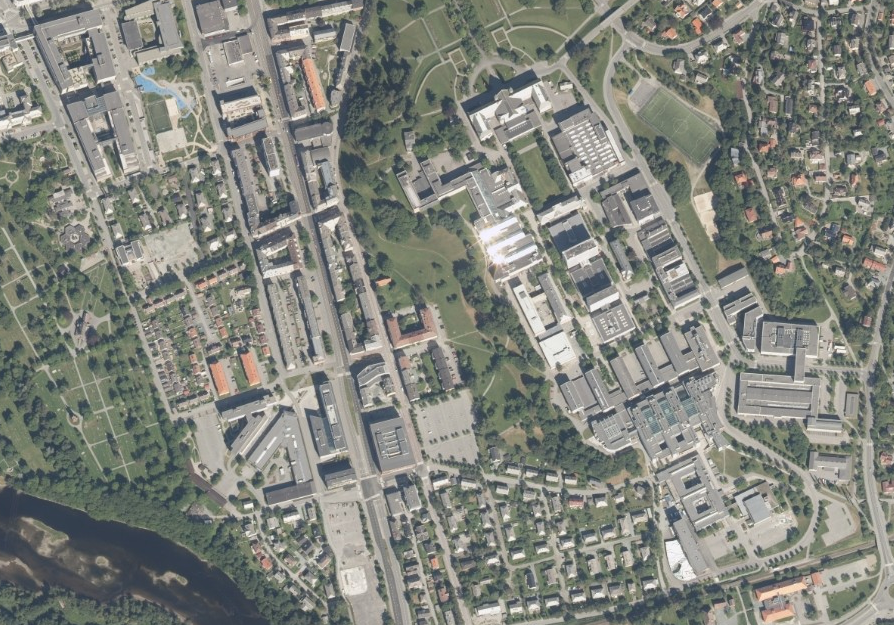
\includegraphics[width=0.8\columnwidth]{figs/aerial_image.png}
\caption[Aerial image]{An aerial image captured above NTNU.}
\label{fig:aerialimage}
\end{center}
\end{figure}

A \ac{CNN} is a special variant of a neural network, where connectivity between units have been constrained and parameter sharing is employed. This will reduce the number of parameters in the model. \ac{CNN}s can, therefore, have many hidden layers, which enables the network to learn a hierarchical representation of the input data. By having a large dataset and conducting normal back-propagation, the network can learn to extract informative features from raw pixel values. \\

This might be well suited for a road extraction system, where there are \todo{is} an abundance of aerial images available covering large areas. Labels can easily be generated for these areas from digital maps stored in a \ac{GIS} database. However, a large issue with utilizing aerial images for training a machine learning algorithm is the presence of noise in the labels. For most purposes, maps can be created without pixel level accuracy and still retain their usefulness. The result is that datasets created from digital maps have some degree of label noise, which can have negative consequences for the accuracy achieved by a machine learning algorithm. \cite{Mnih_aerial_images_noisy} have identified two types of label noise present in aerial images: Omission and registration noise. The former occurs when an object in an aerial image is missing, and the latter happens when there is a misalignment between the object in the image and in the ground truth of the label.\\

One way of reducing the impact of noisy labels is by modifying the loss function. Cross-entropy loss assumes that the labels are correct, which results in noisy labels incorrectly penalizing an accurate classifier. The bootstrapping method proposed by \citep{Reed_noisy_labels_bootstrapping}, utilizes the classifier's implicit knowledge about the task by incorporating the classifier’s predictions in a convex combination with the labels. The quality of these modified targets improves as the classifier's accuracy increases, which is why the method is called bootstrapping.\\

Another compelling way of improving generalization accuracy of a machine learning algorithm, is the use of curriculum learning \citep{Bengio_curriculumlearning}. The method involves organizing the dataset according to a curriculum, where examples are sorted based on a criterion of ``easiness". The examples considered ``easy" are presented early on in the optimization process, whereas ``harder" examples are presented later on.
